

\section{Introduction}
\label{sec:intro}

A memory allocator is a key component that could significantly impact the performance and memory consumption of the corresponding applications. As an example, we evaluated \texttt{PARSEC} applications~\cite{parsec}, \texttt{Phoenix}~\cite{phoenix}, and two stress tests  \texttt{cache-thrash} and \texttt{cache-scatch} from \texttt{Hoard}~\cite{Hoard}, with multiple well-known memory allocators, such as two versions of Linux allocators (\texttt{glibc-2.28} and \texttt{glibc-2.21}), TcMalloc~\cite{tcmalloc}, \texttt{jemalloc}~\cite{jemalloc},  \texttt{Hoard}~\cite{Hoard}, and \texttt{DieHarder}~\cite{DieHarder}. Figure~\ref{fig:motivation} shows performance results of some programs, where all data in the figure is normalized to that of the Linux default allocator (\texttt{glibc-2.28}). We have the following observations: (1)~the performance difference with different allocators can be as large as $38\times$, i.e. \texttt{cache-thrash} with TcMalloc; (2)~No allocator performs consistently the best across all tested applications, indicating the importance of identifying the internal reason.
%, indicating that sometimes spending additional effort toward optimizing the application code may have a smaller  impact than simply switching to a better-suited allocator. (2)~No allocator performs consistently the best across all tested applications, indicating the importance of identifying the internal reason. 

\begin{figure}[!ht]
\centering
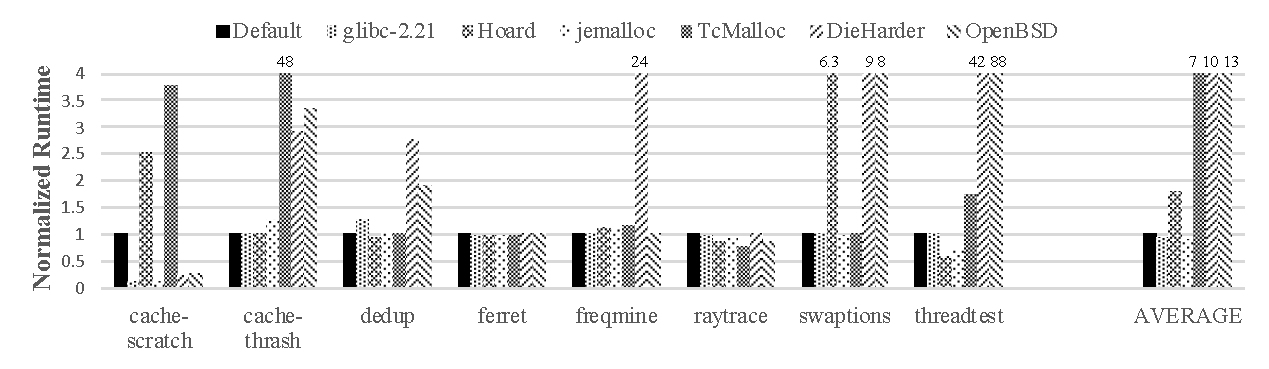
\includegraphics[width=0.98\columnwidth]{figures/motivation}
\caption{Performance Impact of Allocators\label{fig:motivation}}
\end{figure}

\begin{figure}[!ht]
\centering
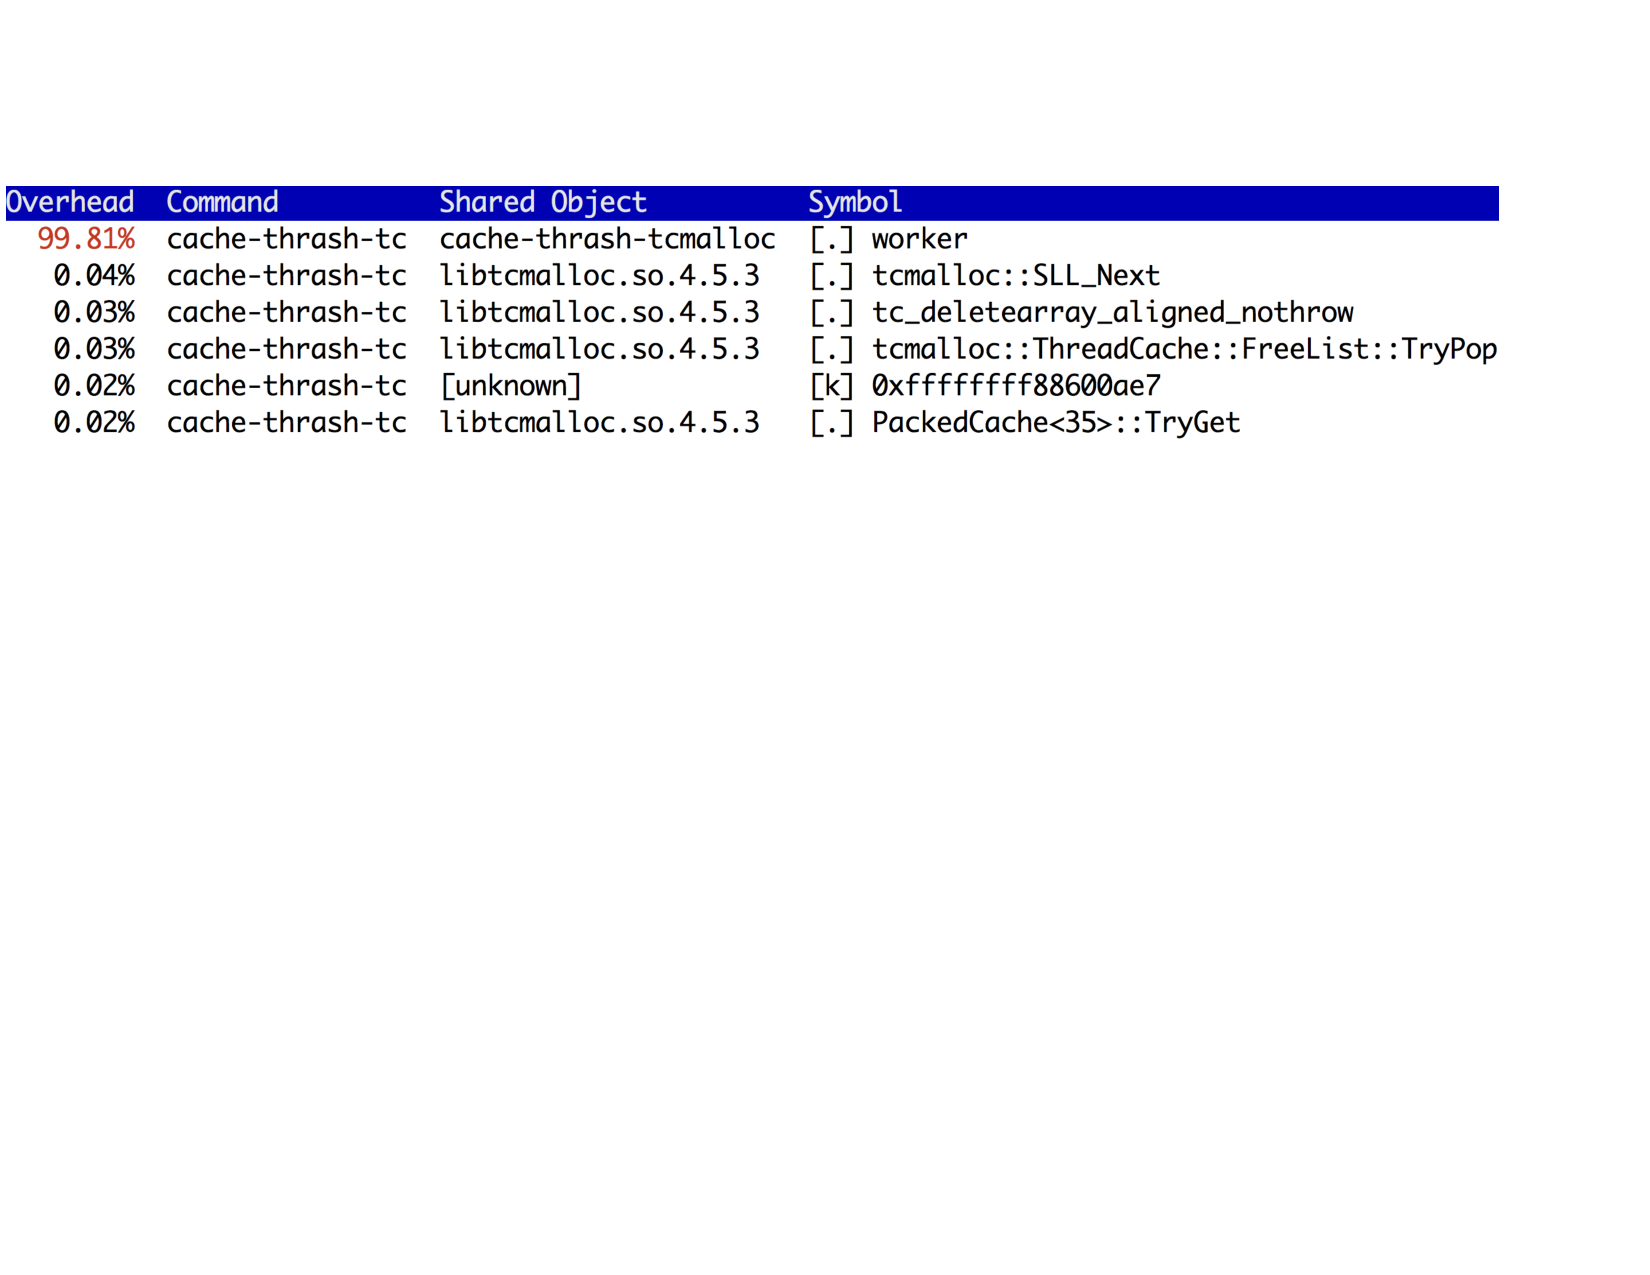
\includegraphics[width=0.9\columnwidth]{figures/perf-cache-thrash-tcmalloc}
\caption{Profiling results of \texttt{perf}. \label{fig:mot1}}
\end{figure}


Due to the obvious importance of a memory allocator, it is emergent to design a profiler that could answer the following questions related to an allocator. \\

\begin{itemize}
\item \textbf{Q1:} \textit{Whether the allocator introduces some performance slowdown for this application? }
\item \textbf{Q2:} \textit{How much the performance can be improved if switching to a well-performed allocator (e.g., TcMalloc)?}
\item \textbf{Q3:} \textit{How much memory wastes the allocator introduces?}
\item \textbf{Q4:} \textit{What are the possible design issues for performance slowdown?}
\item \textbf{Q5:} \textit{What are the reasons for memory wastes?} 
%\item What are quantitative metrics to evaluate a memory allocator? 
\end{itemize}
\vspace{0.1in}

However, \textit{none of existing profilers could answer even one of these questions}. General-purpose profilers like \texttt{gprof}~\cite{DBLP:conf/sigplan/GrahamKM82} and \texttt{perf}~\cite{perf} only report the time accumulation of different functions, and \texttt{Coz}~\cite{Coz} presents a quantitative performance impact of improving a particular region of code. We used \texttt{perf}, \texttt{gprof}, and \texttt{Coz} to analyze the performance issue of TcMalloc on \texttt{cache-thrash}, since it runs around $38\times$ slower than the default Linux allocator. As shown in Figure~\ref{fig:mot1}, \texttt{perf} reports the \texttt{worker} function as the primary function to focus on, which unfortunately has nothing to do with the allocator. \texttt{gprof} reports a similar result as \texttt{perf}. \texttt{Coz} reports lines 85-87 of \texttt{cache-thrash.cpp} as the major issue, and predicts that the performance can be improved up to \textbf{10\%} if these lines can be improved by 100\%. However, it 
also did not pinpoint the real reason for the big slowdown, where TcMalloc's passive false sharing issue introduces a large number of cache invalidations, as discussed in Section~\ref{sec:effectiveness}. 
%In addition, Coz's prediction on the performance impact is misleading (with only 10\%).

%However, they cannot identify the performance issues of a memory allocator, due to the following reasons. \texttt{First}, they do not collect allocator-specific data, and provide no metrics for evaluating an allocator. For instance, \texttt{perf} may report the number of cache misses, but it is impossible to know how many of these events are actually caused by the allocator. Without that information, it is unable to determine whether a performance issue is originating from the allocator. \texttt{Second}, none of these tools collect kernel contention information, an important issue related to the allocator. For instance, the glibc-2.21 allocator slows down the performance of \texttt{dedup} by more than 20\%, which is caused by frequent \texttt{madivse} system calls that directly lead to the heavy kernel contention. However, such an important issue cannot be identified by general profilers~\cite{DBLP:conf/sigplan/GrahamKM82, Coz, perf}%, \todo{as discussed in Section~\ref{}}.
%Third, none of these profilers report the application friendliness of an allocator, which is critical to understanding the performance slowdown caused by a particular allocator.   

Existing allocation profilers, such as \texttt{mprof}~\cite{Zorn:1988:MAP:894814}, Mtrace~\cite{mtrace}, Mtrace++~\cite{Lee:2000:DMM:786772.787150}, TcMalloc profiler~\cite{tcmalloc-profiler}, or CLR profiler~\cite{lupasc2014dynamic}, mainly focus on how an application uses the memory. For instance, \texttt{mprof} attributes memory allocations to different allocation sites, reports memory leaks, and shows the memory usage of functions~\cite{Zorn:1988:MAP:894814}. The TcMalloc profiler reports heap usage of different allocation sites, and locates memory leaks~\cite{tcmalloc-profiler}. That is, these allocation profilers cannot report memory wastes caused by an allocator, which sometimes can be as big as memory consumption of applications. 

This paper presents an allocator profiler--\MP{}--that helps answer all of these questions as listed above. \MP{} will benefit both normal users and allocator designers, since normal users could benefit from answers of the first three questions and allocator designers could utilize it to pinpoint design issues latent inside an allocator (related to \textbf{Q4} and \textbf{Q5}). This profiler  aims to profile different allocators without changing the allocator, so that there is no need to reinvent the wheel for allocator designers, when they design a new allocator or improve an existing allocator. 

In order to answer the question \textbf{Q1}, it is required to understand how an allocator could actually affect the performance of applications. Since an allocator will manage memory allocations and deallocations from applications, it can affect applications in two ways: first, the performance of memory management operations will affect the performance of applications, where slow operations may degrade the performance.  Second, whether an allocator is tapping well with memory usage and access pattern of a particular application, called ``\textit{application friendliness}'' in the remainder of this paper. That is, even a fast allocator could significantly degrade the performance, if it is not tapping well with memory usage pattern of the application. For the previous example, the   high-performant TcMalloc slows \texttt{cache-thrash} by $38\times$ (as shown in Figure~\ref{fig:motivation}) due to its friendliness issue. \MP{} will report application-friendliness of an allocator, including cache utilization rate, page utilization rate, passive/active false sharing, and cache invalidation rate (outside allocations/deallocations), as further described in Section~\ref{sec:profilefriendliness}. 

%in order to reduce the performance overhead. For instance, to collect cache utilization rate, \MP{} tracks used bytes of every cache line, and then updates the overall cache utilization rate upon every sampled access. Overall, these parameters will help users to understand the performance degradation on a specific application. For the previous example, \MP{} reports that the passive false sharing is the direct reason for TcMalloc's low performance on \texttt{cache-trash} application.

It is straightforward to collect the cycles of memory management operations during the execution. Then we propose to replace the collected cycles with those of a target allocator in order to predict the possible performance impact after switching to the target allocator, which helps answer the question \textbf{Q2}. However, there exist multiple issues. The first issue is the accuracy, since the performance for different types of allocations are substantially different (as shown in Table~\ref{tbl:metrics}), such as allocations of small and big objects, serial and parallel phase, new and reused allocations, allocations and deallocations. The second issue is that the target allocator may has different threshold for small and big objects from the current allocator. The third issue is the prediction of multithreaded applications. \MP{} solves all of these issues as discussed in Section~\ref{sec:predict}.

The question \textbf{Q3} is related to memory wastes caused by the allocator. The straightforward method is to intercept memory-related system calls (e.g., \texttt{mmap} and \texttt{sbrk}) inside memory operations to collect the total memory consumption, and then subtract it by  consumption of applications. However, virtual memory is different from physical memory, since physical pages are typically allocated on demand inside the OS. In addition, the allocator may return physical pages to the OS via \texttt{madvise} or \texttt{munmap}. Instead, \MP{} proposes to utilize a page-based mechanism to track memory consumption, where a page is treated as ``allocated'' only when some objects in this page have been allocated to the application. It further tracks \texttt{madvise} and \texttt{munmap} to update memory consumption timely. 

To answer the question \textbf{Q4}, we should understand the reasons of slow memory management operations. Based on our observation, they can be caused by the following reasons. The first reason is due to the complexity of the implementation, which can be measured by the number of instructions inside each operation. The second reason can be caused by hardware events of the algorithm design, such as cache misses. The third reason can be caused by user space contention, which could be evaluated via lock acquisitions and lock contention inside each memory management operation. The fourth reason is due to kernel contention, which could be caused by memory-related system calls. All of these reasons have been observed in different allocators, as further discussed in Section~\ref{sec: benifitdesigners}.  
%and it also introduces multiple cache misses for each free operation. 
%Both DieHarder and Hoard has a high number of lock acquisitions and high contention rate for some applications, and Glibc-2.21 has high kernel contention for \texttt{dedup}. 
Therefore, \MP{} proposes to utilize hardware Performance Monitoring Units (PMUs) to collect the number of instructions and hardware events, and intercepts synchronizations and memory related system calls in order to identify user and kernel space contention. 

For Question \textbf{Q5}, \MP{} reports different types of memory wastes introduced by an allocator. Although it is straightforward to measure internal fragmentation, but not for memory blowup and external fragmentation. Memory blowup occurs when memory deallocations from one thread cannot be utilized to satisfy subsequent memory requests from other threads~\cite{Hoard}, due to the employment of per-thread heaps. However, this definition cannot be utilized directly to collect the total memory blowup, as it does not specify how to update it upon consequent deallocations and re-allocations. \MP{} measures memory blowup with a key observation: \textit{the total size of freed objects represent the upper bound of memory blowup for a size class}. Then the memory blowup can be measured by subtracting the total size with the size of recently-freed objects. After computing the memory blowup, \MP{} is able to compute the external fragmentation afterwards. 



 %\textit{The novelty (and challenge) of \MP{} lies in its decision of what to profile and how to profile precisely and efficiently}, as described in the following. First, \MP{} profiles the performance impact of memory management operations, which will directly affect the performance of running an application. It is straightforward to utilize the time (cycles) of each allocation and deallocation as the metrics, but there exist multiple issues. 
 
 %The second issue is that the runtime itself cannot tell the underlying reason for the performance issue. Instead, \MP{} differentiates the data based on allocation types, such as small/large allocation, new/re-used allocation, which helps identify the real issue inside the allocator. In addition, \MP{} proposes to utilize hardware Performance Monitor Units (PMUs) to collect hardware related events (instructions, cache misses, or page faults), and intercept synchronizations and memory-related system calls to obtain user-space and kernel contention, helping understand the particular design issue inside. For instance, glibc-2.21 invokes a large number of \texttt{madvise} system calls for the \texttt{dedup} application~\cite{madvise}, where the system call overhead and unnecessary page faults are the major reason of 28\% slowdown. 
%\MP{} is able to report such issues by intercepting memory-related system calls. 

Overall, \MP{} profiles multiple important aspects of memory allocators, such as performance, memory, scalability, and application-friendliness. Based on our extensive evaluation, \MP{} successfully identifies multiple known and \textbf{unknown} design issues inside popular allocators, as further described in Section~\ref{sec:effectiveness}. Due to its careful design, \MP{} only imposes 35\% performance overhead on average. This efficient design reduces \MP{}'s interference to the original execution. \MP{} does not need the change of the allocator, the application, and the underlying OS, which will be convenient for the employment. 

%\todo{one way to highlight the contribution is to emphasize on the **complex** considerations of designing good allocators and the challenges to identify design problems. We want to let the reviewer know that it's difficult to do. }

\subsection*{Contribution}

Overall, this paper makes the following contributions. 

\begin{itemize}
\item \MP{} is the first systematic approach to evaluate and profile different memory allocators, without changing the internal implementation of allocators. More specifically, \MP{} proposes the combination of function interception (based on common APIs) and PMU-based sampling to perform the profiling.

%It proposes the first general profiler--\MP{}--to profile different memory allocators, without the need of the change of the allocator and the underlying OS, if an allocator utilizes the standard synchronization and system calls.  

\item \MP{} analyzes multiple relevant factors that an allocator may impact the performance of applications.
%important reasons that may impact  of an allocator that will significantly impact the performance and memory overhead of an allocator, with the assistance of PMUs, time-stamp counters, and simple counters together. 

\item \MP{} proposes the first experimental mechanisms to quantitatively measure memory blowup (and external fragmentation), cache/page utilization rate, and passive/active false sharing impact. 
%, multiple practical methods to profile some metrics precisely and efficiently for the first time, such as memory blowup, . 
%profile cache/page utilization rate, memory blowup, active/passive false sharing, and kernel contention for the first time.
%, and attributes the data to each allocation and deallocation, helps discover designing issues that cannot be discovered with general profilers.  
%\item \MP{} proposes a practical method to predict the performance impact of the current allocator, which allows normal users to 
\item This paper performs extensive experimentation to confirm \MP{}'s effectiveness and overhead. The experiments also uncovers multiple known and unknown design issues in widely-used allocators.  

\end{itemize} 

\begin{comment}

%\todo{What is new in this tool? Whether it could provide some information that is not available in an existing allocator.}

\begin{itemize}
\item It will quantify application-friendliness, which is not available in existing work, and which helps users to decide which allocator should be used for a specific application. 
\item It will provide the memory usage (overhead) information, such as internal fragmentation, and objects that are not freed but yet which remain unused. 
\item It will provide some information that only exists across multiple profilers, for instance, the average number of instructions of each allocation and deallocation, the average time spent within each allocation and deallocation (PMU sampling will be placed outside of the time span, thus not avoiding an erroneous measurement of how long this allocation and deallocation request has been sampled), whether there are some contentions during allocation (user space and kernel space), how many lock acquisitions.  
\end{itemize}
 	
\end{comment}

\subsection*{Outline}

The remained of this paper is organized as follows. Section~\ref{sec:background} discusses the background of memory allocators, and the basic idea and challenges of \MP{}. Then Section~\ref{sec:implementation} presents the detailed implementation. After that, Section~\ref{sec:evaluation} shows the results of experiments on different allocators using \MP{}, and Section~\ref{sec:limitation} discusses some limitations. In the end, Section~\ref{sec:relatedwork} discusses related work in this field, and Section~\ref{sec:conclusion} concludes this paper.